\documentclass[preprint]{aastex} 

\usepackage[top=1in, bottom=1in, left=1in, right=1in]{geometry}
\usepackage{amsmath}
\usepackage{graphicx}
\usepackage{mdwlist}
\usepackage{natbib}
\usepackage{natbibspacing}
\setlength{\bibspacing}{0pt}
\setlength{\parskip}{0pt}
\setlength{\parsep}{0pt}
\setlength{\headsep}{0pt}
\setlength{\topskip}{0pt}
\setlength{\topmargin}{0pt}
\setlength{\topsep}{0pt}
\setlength{\partopsep}{0pt}
\setlength{\footnotesep}{8pt}
\pagestyle{empty}
\citestyle{aa}

%Project Description (8-pages maximum), including the following:
%- A statement of which of the four categories of MSIP is most appropriate
%for this proposal as the first sentence (see section II. Program Description).
%- A scientific justification. For Open Access Capabilities, explain the
%uniqueness and lack of general availability of the capability.
%- A description of the broader impacts, including student training.
%- A description of benefits to the community (observing time, data products, etc.)
%- An outline of the project management plan (where appropriate).
%Note: Results from Prior NSF Support should not be included. Links to URLs may
%not be used.

\begin{document}
\title{HERA}

% XXX A statement of which of the four categories of MSIP is most appropriate
%for this proposal as the first sentence (see section II. Program Description).

\section{Scientific Justification}

Our proposal is directed toward the science of cosmic reionization--the rapid 
ionization of the majority of the hydrogen
in the universe by the light of the first stars and supermassive black
holes (Furlanetto et al. 2006).  
% XXX allude to decadal survey
The HERA program was the highest ranked of the Decadal Survey RMS Panel
scientific recommendations (A2010 Panel Reports).

\subsection{\it Our Understanding of Cosmic Reionization}
Modern cosmology predicts the existence of a mostly neutral IGM 
lasting from cosmic recombination until the first luminous
objects ionized it between 300 and 800Myrs after the Big Bang.
Redshifted emission from the 21cm hyperfine transition of neutral hydrogen provides a
unique tracer of the primordial IGM.   Variations in this signal
versus redshift and direction could be reconstructed into a
three-dimensional map of the evolution of cosmic structure (Furlanetto et al.
2006).  The direct observation of the neutral IGM via this signal
would be an achievement comparable with
the discovery of the Cosmic Microwave Background (CMB).

Recent observations of Gunn-Peterson absorption by the IGM
toward the most distant quasars and the
large-scale polarization of the CMB indicate that reionization was a
complex process starting
perhaps as early as $z \approx 14$, with the last vestiges of the the
neutral IGM being etched-away by $z \approx6$ (Fan et al. 2006; Page
et al. 2007; Becker et al. 2001).  Unfortunately, both of these
ground-breaking results are limited in diagnostic capabilities: the Gunn-Peterson
effect saturates at low neutral fractions, and the CMB polarization only provides
an integral measure of the Thompson optical depth back to
recombination.

The HI 21 cm signal depends on a number of factors such as 
the evolution of the matter density power spectrum,
the efficiency of ionizing photon production in early galaxies,
the effect of X-ray, shock, and Ly$\alpha$ heating on 
the thermal balance between the CMB and the
kinetic and spin temperatures of gas in the IGM, and the
feedback of this heating on star formation.
Hence, study of the evolution
of the neutral IGM provides a rich physical data set that constrains
the nature and distribution of the first luminous sources, early large
scale structure formation, and radiative processes in the early
Universe (Morales et al. 2010). It comes with no surprise that the Decadal
Survey 
Report called out the probing of this last unexplored vista of cosmic
evolution as one of the ``primary areas with extraordinary discovery
potential'' in astrophysics in the next decade (A2010).

Over the past decade, cosmologists have focused extensively on modeling of reionization.
Fig. \ref{fig:eor_cut_mcquinn}
shows a recent simulation of HI 21 cm emission during reionization
(McQuinn 2010, unpublished) that is typical of the growing
sophistication of such models (Santos et al. 2010; Mesinger et
al.  2010; Zahn et al. 2010; Wyithe et al. 2004), and is unique for
spanning much of PAPER's redshift and spatial coverage.
Three-dimensional tomographic imaging of how temperature fluctuations
grow and are erased by ionization will require a collecting area
comparable to a full Square Kilometer Array (SKA). However, detecting
the fluctuating 21 cm signal from the IGM prior to a full SKA is still
possible statistically through power spectrum analysis, in direct
analogy to the statistical discovery of CMB fluctuations by COBE.

\begin{figure}[!ht]\centering
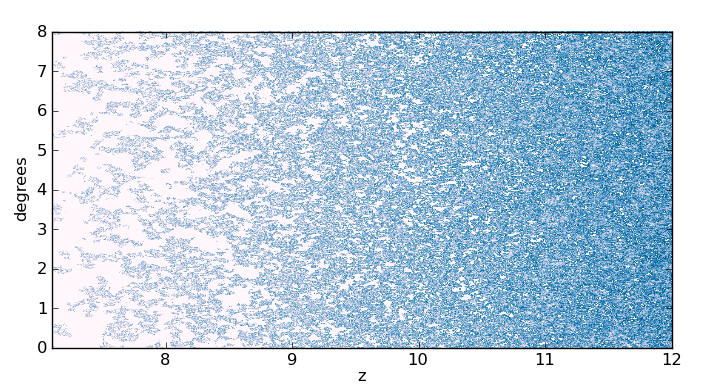
\includegraphics[height=3in]{plots/dens_ion_slice_v5.png}
\caption{Shown above is a large-scale simulation of 21 cm brightness
  temperature of HI, accounting for evolution in ionization fraction
  (McQuinn 2010).  At high redshift ($z=12$; 106MHz), brightness
  temperature tracks gas density.  As density fluctuations grow, UV
  photon production outpaces recombination, and regions become
  ionized (white). At the end of the era ($z=7$; 177MHz) only the
  rarest regions have any remaining neutral hydrogen.  Large simulation
  volumes and continuous redshift coverage from $z=6$ to $z=12$ are key elements of
  simulations relevant to PAPER.  }
\label{fig:eor_cut_mcquinn}
\end{figure}

\subsection{\it{HERA Objectives}}

\subsection{\it{In the Context of the HERA Road Map}}

\subsection{\it{Content of the Proposal}}

\section{The HERA Instrument and Signal Flow}

\section{Reionization Science}

\subsection{\it{Power Spectrum Measurements}}

\subsection{\it{Foreground Characterization}}

\section{Broader Impact of Our Activities}

\subsection{\it Instrument Development and Analysis Techniques}

\subsection{\it Student Training}

\subsection{\it Benefits to the Community}

\subsection{\it Preparations for HERA II}

\end{document}

